% Created 2019-11-17 dom 12:05
% Intended LaTeX compiler: pdflatex
\documentclass[11pt]{article}
\usepackage[utf8]{inputenc}
\usepackage[T1]{fontenc}
\usepackage{graphicx}
\usepackage{grffile}
\usepackage{longtable}
\usepackage{wrapfig}
\usepackage{rotating}
\usepackage[normalem]{ulem}
\usepackage{amsmath}
\usepackage{textcomp}
\usepackage{amssymb}
\usepackage{capt-of}
\usepackage{hyperref}
\setlength{\parindent}{0in}
\usepackage[margin=1.0in]{geometry}
\usepackage{mathtools}
\author{Luis Antonio Ortega Andrés  \\Guillermo Galindo Ortuño  \\ Johanna Capote Robayna}
\date{}
\title{Memoria técnica}
\hypersetup{
 pdfauthor={Luis Antonio Ortega Andrés  \\Guillermo Galindo Ortuño  \\ Johanna Capote Robayna},
 pdftitle={Memoria técnica},
 pdfkeywords={},
 pdfsubject={},
 pdfcreator={Emacs 26.3 (Org mode 9.3)}, 
 pdflang={English}}
\begin{document}

\maketitle

\section{Estructura del proyecto}
\label{sec:orgcea4ad5}

La aplicación \texttt{Alamabra1925} está implementada como un proyecto \texttt{Android} en \texttt{Kotlin}.
El proyecto se encuentra estructurado en una única actividad \texttt{MainActivity} y una serie de fragmentos, cada uno de ellos encargado de una faceta de la aplicación.
Estos son:
\begin{itemize}
\item \texttt{HomeFragment}.
\item \texttt{InnerMapListFragment}.
\item \texttt{InnerMapFragment}.
\item \texttt{InterestPointFragment}.
\item \texttt{InterestPointMenuFragment}.
\item \texttt{GameFragment}.
\end{itemize}

Todos los fragmentos y las interacciones entre ellos se llevan a cabo utilizando un ``controlador de navegación''. Este nos permite navegar entre los fragmentos desde la barra de navegación lateral. 

Desde esta barra podemos acceder a \texttt{HomeFragment} (Map), \texttt{InnerMapListFragment}
(Inside Maps) y \texttt{GameFragment} (Game).

A continuación mostramos el diagrama correspondiente a las comunicaciones entre cada uno de los fragmentos. 

\begin{center}
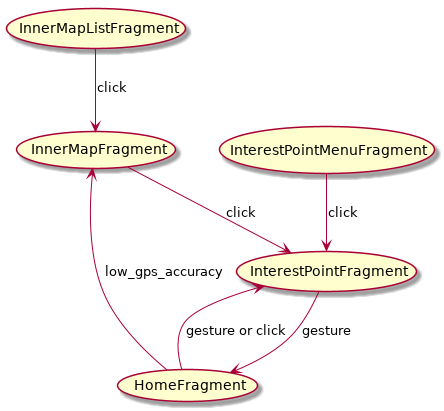
\includegraphics[width=.9\linewidth]{./diagrama1.png}
\end{center}


Simbolizaremos con flechas continuas la cantidad de veces que una clase contiene a la otra. Debido a la estructura con fragmentos del proyecto esto solo ocurre con la clase \texttt{InterestPointMenuFragment}. Por esto, hemos decidido simbolizar en el diagrama las comuninaciones entre las clases. Para ello usaremos lineas discontinuas.

\begin{center}
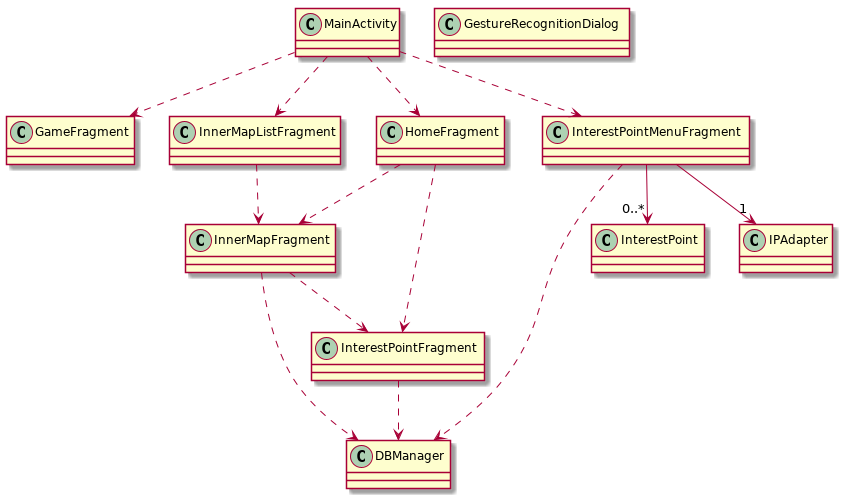
\includegraphics[width=.9\linewidth]{./diagrama2.png}
\end{center}


\section{Fragmentos}
\label{sec:orge6f137c}
\subsection{HomeFragment}
\label{sec:org6f24e37}

\subsection{InnerMapFragment}
\label{sec:org8240bf4}

\subsection{InnerMapListFragment}
\label{sec:orgedf9294}

\subsection{InterestPointFragment}
\label{sec:org27f78a3}

Este fragmento nos permite visualizar toda la información acerca de un punto de interés concreto de nuestra visita. 
En el método \texttt{onCreateView} del fragmento, esperamos un \texttt{Bundle} con un identificador que nos permita conocer de que fragmento se debe mostrar la información.

Con esto utilizamos la base de datos para rellenar los \texttt{textView} apropiados.

\subsection{InterestPointMenuFragment}
\label{sec:orge7ed27d}

A este fragmento se puede acceder desde la barra de navegación lateral bajo el nombre de \texttt{Interest Points Menu}. Aquí obtendremos una lista de todos los puntos de interés de os que se tiene información en la aplicación. Para ello utilizamos un adaptador \texttt{IPAdapter} y la base de datos.

Cada uno de los puntos de la lista tiene sobrecargado el listener de pulsación, haciendo que sea posible ir a la vista detallada de cada uno de ellos.

En el método \texttt{onCreateView} hacemos lo siguiente.

\begin{verbatim}
    val mainList = root.findViewById<ListView>(R.id.list_view)
    listAdapter = IPAdapter(this.context!!, list)
    mainList.adapter = listAdapter

    mainList.onItemClickListener = AdapterView.OnItemClickListener { _, _, position, _ ->
        val bundle = bundleOf("id" to list[position].id)
        findNavController().navigate(R.id.action_nav_ip_menu_to_nav_ip, bundle)
    }
    
    loadQueryAll()
\end{verbatim}

\begin{itemize}
\item Inicializamos la variable correspondiente a la vista de la lista.
\item Inicializamos nuestro adaptador. Y se lo asignamos a la lista.
\item Sobrecargamos el listener de pulsación de forma que utilice controlador de navegación para cargar el fragmento del punto de interés correspondiente.
\item Utilizamos \texttt{loadQueryAll} para rellenar la lista con los puntos de interés de la base de datos.
\end{itemize}

\subsection{GameFragment}
\label{sec:org0e10f51}

En este fragmento el usuario se enfrenta a una serie de preguntas que tendrá que responder lo más rápido posible. 

\section{Otras clases}
\label{sec:org22d57bb}

\subsection{InterestPoint}
\label{sec:orgfae7d2e}

Esta clase corresponde a una simple abstracción de la información almacenada en un punto de interés.

\begin{verbatim}
data class InterestPoint(
        var id : Int,
        var title: String,
        var content : String
)
\end{verbatim}


\subsection{IPAdapter}
\label{sec:orgbd7fca9}

Esta clase extiende a la clase \texttt{BaseAdapter}. La utilizamos en el fragmento correspondiente a la lista de puntos de interés \texttt{InterestPointMenuFragment} donde mostramos uan lista de todos los puntos de interes que se encuentran en la base de datos.
El adaptador nos permite mostrar estos elementos en la lista de una forma más cómoda y personalizable. Podriamos haber utilizado un \texttt{ArrayAdapter} como se ha hecho en la lista de mapas interiores \texttt{InnerMapListFragment}, sin embargo, esto bloqueaba la escalabilidad de la aplicación a la hora de querer mostrar mas información en la lista (por ejemplo, imágenes o un resumen del contenido).


\subsection{DBManager}
\label{sec:org292ad2b}

Esta clase nos permite utilizar la API de \texttt{SQLite} para almacenar los puntos de interés de nuestra aplicación. Dado que estos no cambian a lo largo de la ejecución podríamos haber utilizado un vector que los almacenara, sin embargo, vimos mas conveniente este modelo, debido a que todos los fragmentos se pueden valer de la misma base de datos (por tener solo una actividad) y no tenemos que preocuparnos de tener un vector al que todos pudieran acceder.

La información almacenada en la base de datos es:
\begin{itemize}
\item Un identificador numérico. La clave primaria.
\item El nombre del punto de interés.
\item Toda la información al respecto del mismo.
\item Su possición.
\begin{itemize}
\item Se utiliza un valor numérico para indicar si el punto de interes se encuentra en el interior o dentro de algún edificio.
\item En el caso de ser un punto exterior, se utilizan latitud y longitud para determinarla.
\item En caso de ser un punto interior, se utilizan un sistema de márgenes para posicionarlo en el mapa.
\end{itemize}
\end{itemize}

La clase dispone de 3 métodos importantes, todos ellos nos devuelven un cursor iterable sobre las filas resultantes en la base de datos.

\begin{itemize}
\item \texttt{queryById}. Nos permite obtener un punto de interés a partir de su ID.
\item \texttt{queryByLocationType}. Nos permite obtener todos los puntos de interés que se encuentren en el exterior o dentro de un mismo edificio.
\item \texttt{queryAll}. Nos permite obtener todos los puntos de interés.
\end{itemize}

\subsection{GestureRecognitionDialog.}
\label{sec:org2c169d5}
\end{document}
